
\documentclass[11pt]{article}
\usepackage[margin=.8in]{geometry}
\usepackage{amsmath,amssymb,amsthm, latexsym, mathrsfs, pdfsync, multicol,
%setspace,
%graphics, 
fancybox, fancyhdr,
graphicx, enumerate,
subfig, tikz, pgfplots,array,tabularx}

%\singlespacing
\def\RR{{\mathbb R}}
\def\NN{{\mathbb N}}
\def\ZZ{{\mathbb Z}}
\def\QQ{{\mathbb Q}}
\def\CC{{\mathbb C}}
\def\bc{\begin{center}}
\def\ec{\end{center}}
\def\be{\begin{enumerate}}
\def\ee{\end{enumerate}}
\def\bi{\begin{itemize}}
\def\ei{\end{itemize}}
\def\bs{\begin{slide}}
\def\es{\end{slide}}
\def\bx{\begin{exercise}}
\def\ex{\end{exercise}}
\def\t{\times}
\newcommand{\ol}[1]{\overline{#1}}
\newcommand{\oimp}[1]{\overset{#1}{\Longleftrightarrow}}
\newcommand{\bv}[1]{\ensuremath{ \mathbf{\vec{#1}}} }
\renewcommand{\d}{\displaystyle}
\newcommand{\blank}[1]{\rule{#1}{0.75pt}}

\usetikzlibrary{calc}

%for tikz pictures
\pgfplotsset{compat=1.6}

\pgfplotsset{soldot/.style={color=black,only marks,mark=*}} \pgfplotsset{holdot/.style={color=black,fill=white,only marks,mark=*}}
\pgfplotsset{my style/.append style={axis x line=middle, axis y line=middle, xlabel={$x$}, ylabel={$y$}}}


%
% Answerbox:
%
%\newcommand\answerbox[3]{#3 \fbox{\rule{#1}{0cm}\rule{0cm}{#2}}}
%
%\setlength{\headsep}{2pt}

\lhead{\sc{Math 251 Calculus I}}
\chead{\large \sc Midterm II} 
\rhead{\sc Fall 2019}
\cfoot{}
\pagestyle{fancy}
%
\begin{document}
\thispagestyle{fancy}

\vspace{.1in}
\begin{tabular}{l@{\hspace{.4in}}l}
Your Name & Your Signature\\
\framebox(200,30){} & \framebox(200,30){} \\
\end{tabular}

%\bigskip

\begin{tabular}{l@{\hspace{.4in}}l}
Instructor Name & \\
\framebox(200,30){}&  \\
\end{tabular}
{
\renewcommand{\baselinestretch}{1.8}
\setlength{\tabcolsep}{.2in}
\normalsize
\begin{center}
\begin{tabular}{|c|c|c|}
\hline
Problem&Total Points&\parbox{.8in}{\hfil Score\hfil}\\
\hline
1&8&\\
\hline
2&14&\\
\hline
3&12&\\
\hline
4&10&\\
\hline
5&16&\\
\hline
6&14&\\
\hline
7&12&\\
\hline
8&14&\\
\hline
\hline
Extra Credit & (5) & \\
%\hline
\hline
Total&100&\\
\hline
%Current Course Grade&\multicolumn{2}{c|  }{}\\
%\hline

\end{tabular}

\end{center}
}
\begin{itemize}
\item 
This test is closed notes and closed book. 

\item You may \textbf{not} use a calculator.

\item
In order to receive full credit, you must {\bf show your work.}  
Be wary of doing computations in your head. Instead, write out your
computations on the exam paper.
 
\item
Raise your hand if you have a question.

\end{itemize}

\newpage
\vspace*{-0.3in}
\begin{enumerate}
%%%Linearization
\item (8 points)

\begin{enumerate}

\item Find the linearization of $f(x) = \sqrt[3]{x}$ at $a = 8$.

\vfill

\item Use your result in part (a) to approximate $\sqrt[3]{7}$.
\vfill
\end{enumerate}
\newpage
%%%Related Rate
\item (14 points) A ladder 12 ft long is propped against a wall. At the moment the ladder makes a 60$^\circ$ angle to the ground, the bottom of the ladder is moving at a rate of 2 ft/sec away from the wall.

\begin{tikzpicture}
\draw (0,5) -- (0,0) -- (6,0);
\draw[ultra thick] (0,4) -- (2.8,0);
\node at (2.1,0.4){\large{$\theta$}};
\node at (1.4,-0.4){\large{$a$}};
\node at (-.4,2){\large{$b$}};
\end{tikzpicture}

Find the rate at which the top of the ladder is sliding down the wall at this same moment. Include units in your answer.

\vskip1in

\newpage

%%% Questions about f(x) given a graph of its derivative
\item (12 points)


The graph of the \textit{\textbf{derivative}} $f'$ of a function $f$ is shown.

\begin{tikzpicture}
\begin{axis}[scale=1.2, my style, xtick={-7,-6,-5,-4,...,5}, ytick={-4,-3,...,4},
xmin=-7, xmax=5, ymin=-4, ymax=4, minor y tick num=0,
minor x tick num=0, mark size=5.0pt,
grid=both, ylabel=$f'(x)$,samples=60]
\addplot[domain=-5.4:4.85, <->, ultra thick] {-(-x+2)^2*(-x-4)/20};
% \addplot[only marks, mark size=2pt] coordinates {(0,-1.8) (7,2.4)};
\end{axis}
\end{tikzpicture}
\begin{enumerate}
\item Determine the critical points of $f(x).$\\
\vfill
\item On what intervals is $f$ increasing or decreasing? Use interval notation.\\
\vfill
\item At what values of $x$ does $f$ have a local maximum or minimum?\\
\vfill
\item On what intervals is $f$ concave up or concave down? Use interval notation.\\
\vfill
%Or just 2 of these!
\end{enumerate}
\newpage
%%%%%Problem: Implicit Differentiation and Tangent Line
\item (10 points) 
Consider the curve given by the implicitly defined function
\[ x^2-x y+3y^2=9 \]

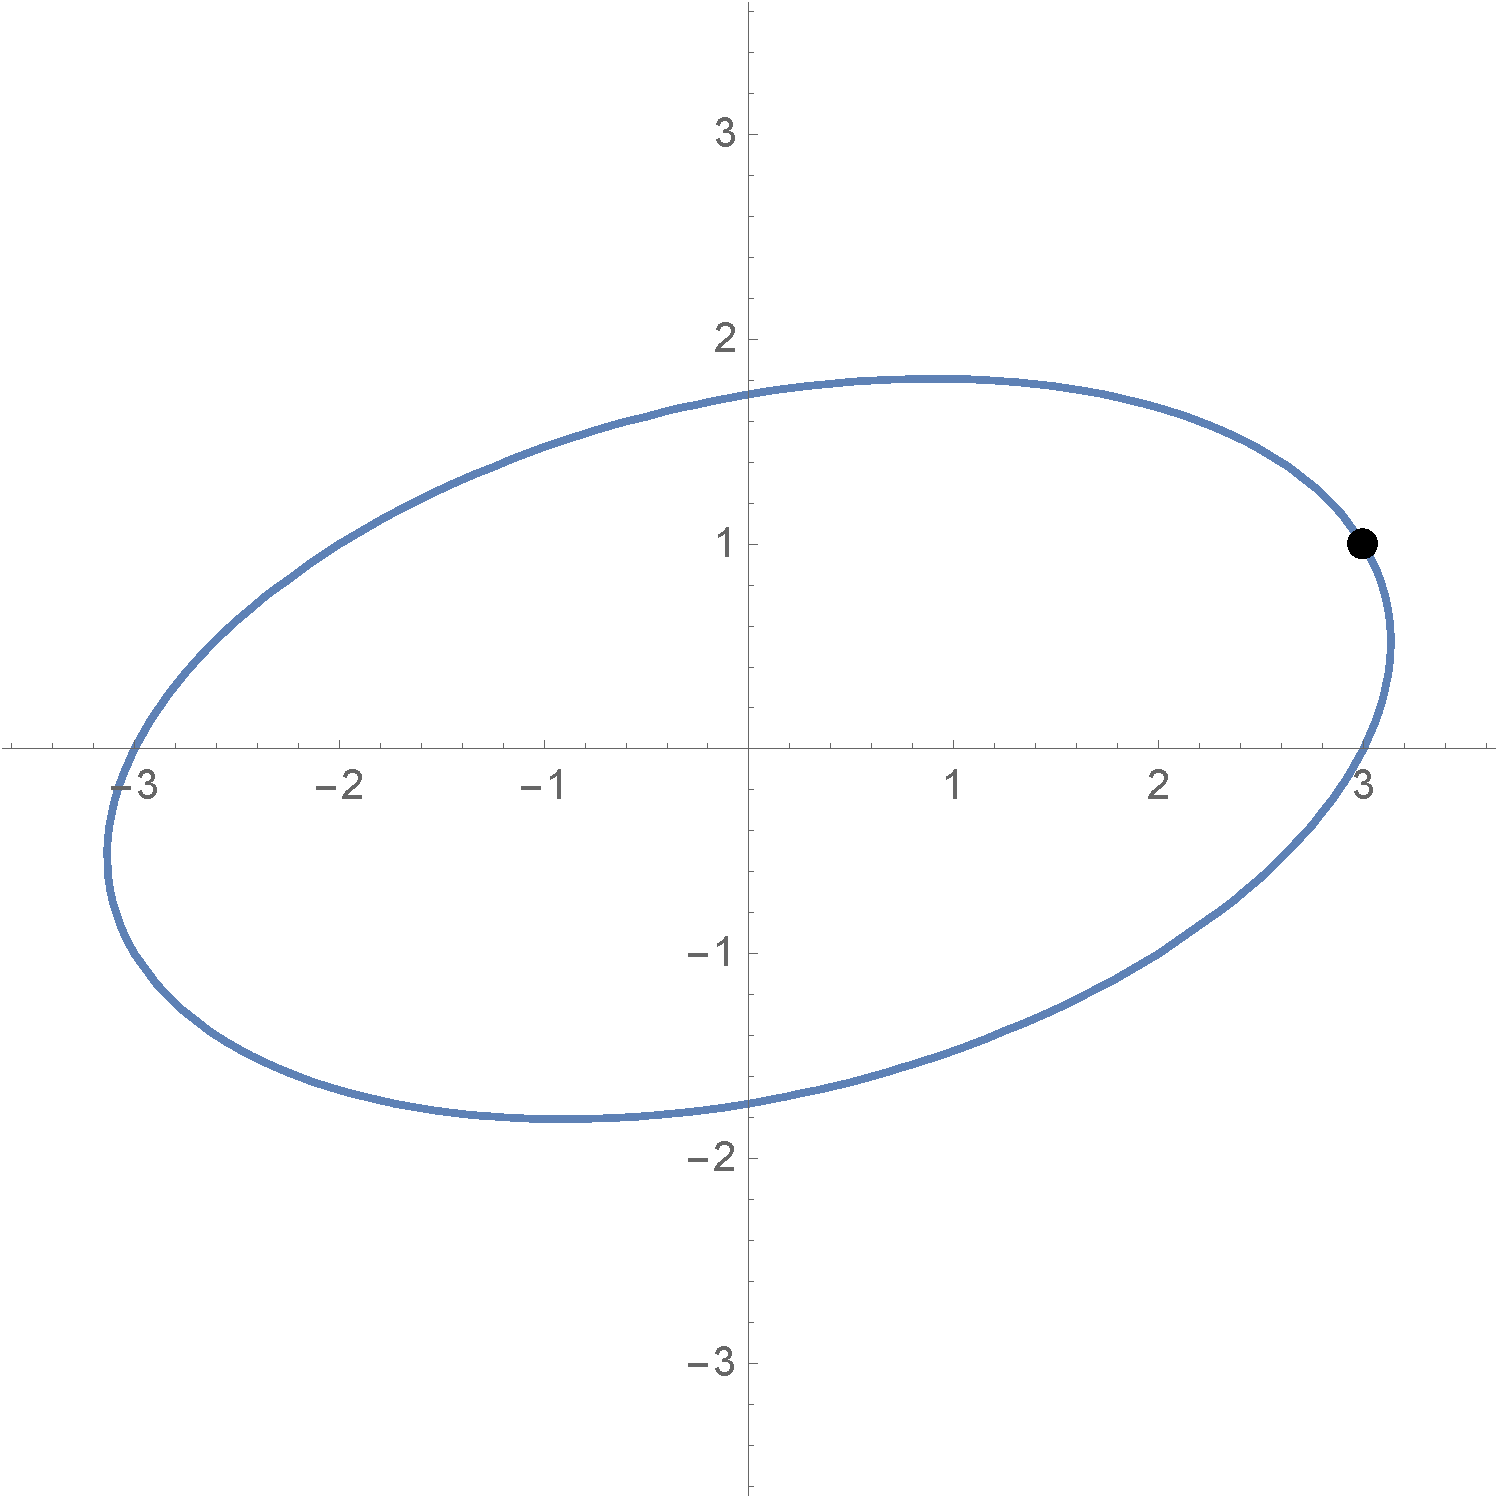
\includegraphics[width=.4\linewidth]{ImpDifPlot}
\begin{enumerate}
\item On the figure above, sketch the tangent line to the curve at the point $(3,1).$\\

\item Find the equation of the tangent line to the curve at the point $(3,1)$ (shown on the picture by the solid dot).\\
\vfill
\end{enumerate}

\newpage
%%%%%Problem: Sketch a curve given some information

\item (16 points) We want to sketch a graph of a function $f(x)$ with certain specified properties.

\begin{enumerate}
\item Fill in the following tables. (You can use words or pictures.)

\renewcommand{\arraystretch}{1.8}
\begin{tabular}{| c | l |} \hline
function information & \quad \hspace{1.5cm} what you conclude about the behavior of $f$\hspace{1.5cm} \quad\\ \hline \hline
 $\lim\limits_{x \to 0^-} f(x) = \infty$ & \\ 
 $\lim\limits_{x \to 0^+} f(x) = -\infty$ &\\ \hline
 $\lim\limits_{x \to - \infty} f(x) = -\infty$  & \\ \hline
 $\lim\limits_{x \to  \infty} f(x) = 2$  & \\ \hline
 $f(1) =0$ & \\ \hline
 $f'(3) =  0$ & \\ \hline
\end{tabular}

\bigskip

\begin{small}
\begin{tabular}{| l || c |  c | c | }
\hline
 $x$  &\quad $-\infty< x<0$ \quad \quad &\quad  $0 < x <3$ \quad \quad & $3 < x < \infty$  \\ \hline
 sign of $f'(x)$ & $+$  & $+$  & $-$     \\ \hline
Behavior of $f(x)$& &&\\ \hline
  \end{tabular}
  \end{small}
  
  \begin{small}
\begin{tabular}{| l || c | c | c | }\hline
 $x$  &\quad $-\infty< x<0$ \quad \quad& \quad \hspace{.1in}\quad$0< x < 4$ \quad  \hspace{.1in} \quad& $4 < x < \infty $ \\ \hline
 sign of $f''(x)$ & $+$ & $-$ & $+$  \\ \hline
Behavior of $f(x)$& &&\\\hline
  \end{tabular}
  \end{small}

% $f''(x) < 0$ on $(-3, 4), (4, 8)$ \\ \hline
% $f''(x) > 0$ on $(-\infty, -3), (8, \infty)$ \\ \hline


\item  Sketch the graph of $f$ that has all of the properties listed in the tables. Label \fbox{{\bf on the graph}}  any local maxima and minima,  any inflection points, any horizontal asymptotes and vertical asymptotes (draw with dashed lines, label with their equations), and any roots of the function that were specified in the table. {\bf Label the axes (add tick marks) to indicate important $x$- and $y$-values.} Your sketch does not need to be to scale.


\vfill
\begin{tikzpicture}
\draw (0,-3)-- (0,5);
\draw (-5, 0) -- (10,0);
\end{tikzpicture}

\end{enumerate}
\newpage
%%%%%Problem: Find maxima and minima, given a polynomial
\item (14 points) Consider the function $g(x) = 2 x^5+5 x^4-10 x^3+2$. 
\be
\item Determine all critical values of $g(x)$ and identify each value as the location of a local maximum, a local minimum, or neither. Justify your answer. 
\vspace{3.5in}
\item  Consider $g(x)$ on the interval $[-1,2]$. Determine the absolute maximum and minimum for $g(x)$ on that interval. (Hint: $g(2) = 66$)\\
\vfill
\item Below is a computer-generated plot of $g(x)$ on the intervals $[-10,10]$. Does this plot contradict your previous answers? Briefly explain.

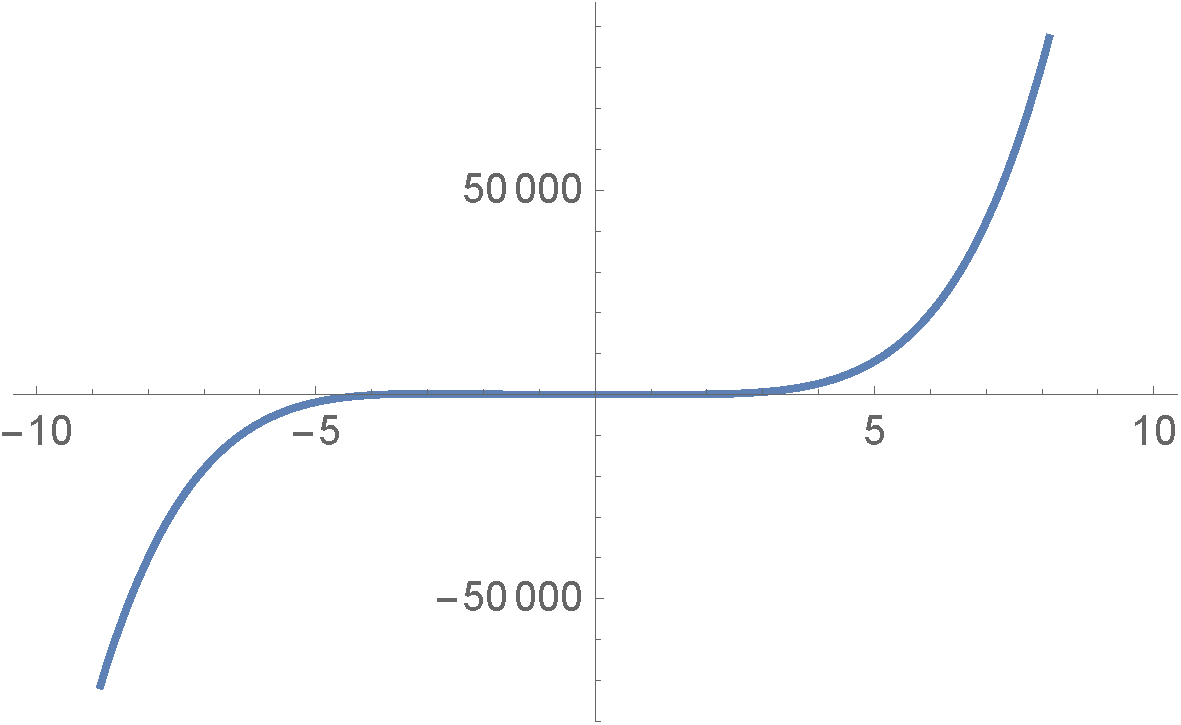
\includegraphics[width=.45\textwidth]{g(x)[-10,10]}\\

\ee
\newpage
%%%%%%%%%%%L'Hopital's Rule
\item (12 points) Evaluate the limits below. Indicate a use of L'H\^{o}pital's Rule by a symbol (such as \textbf{L'H} or \textbf{H}) over the equal sign. 
	\begin{enumerate}
	\item $\d{\lim_{t \to 3} \frac{\sin(\pi t)}{t^2-9} }$
	\vfill
	\item $\d{\lim_{x \to 0 } \frac{x-5\cos(\pi x)}{4e^x} }$
	\vfill
	\item $\d{\lim_{x \to \infty} x(8-8e^{\frac{1}{x}})}$
	\vfill
	\end{enumerate}
\newpage
%%%Optimization
\item (14 points) A box with a square base must have a volume of 2500 $\text{in}^3.$ Wood for the base and sides costs $ \$0.50$ per square inch and wood for the decorative top costs $ \$2$ per square inch. What are the dimensions of the least expensive box?
\begin{enumerate}
\item Draw and label a picture.
\vspace{1.5in}
\item Explicitly state what it is you must minimize or maximize. (One or two words is sufficient.)
\vspace{.5in}
\item Write the quantity in part (b) as a function of one variable and state its domain.
\vfill
\item Answer the question and justify your answer.
\vfill
\end{enumerate}
\end{enumerate}
\newpage
\textbf{Extra Credit:} (5 points) Is the statement below TRUE or FALSE? Justify your answer.
 \begin{quote} Suppose $t >0.$ An antiderivative of $$\d f(t) = \arcsin\left(\frac1t\right) - \frac{1}{\sqrt{t^2 - 1}}$$  is 
$$\d
F(t) = t\arcsin\left(\frac1t\right) - 4.
$$
\end{quote}

\end{document}
